\documentclass[11pt,a4paper]{article}

% ---------------------------------------------------------------- paquetes
\usepackage[utf8]{inputenc}
\usepackage[T1]{fontenc}
% es-noshorthands: evita que babel active < > " , que chocan con TikZ y siunitx
\usepackage[spanish,es-nodecimaldot,es-noshorthands]{babel}
\usepackage{lmodern}
\usepackage{microtype}
\usepackage[a4paper,top=2.6cm,bottom=2.6cm,left=2.7cm,right=2.7cm]{geometry}
\usepackage{amsmath,amssymb}
\usepackage{siunitx}
\usepackage{graphicx}
\usepackage{booktabs}
\usepackage{xcolor}
\usepackage{caption}
\usepackage{tikz}
\usetikzlibrary{arrows.meta,patterns,calc}
\usepackage{fancyhdr}
\usepackage[hidelinks]{hyperref}

% ------------------------------------------------------- color corporativo
% Ajusta este RGB al verde exacto de la UJI si el tuyo es otro.
\definecolor{uji}{RGB}{0,104,71}

% ------------------------------------------------- referencias y rotulado
\newcommand{\cita}[1]{\textsuperscript{[\textcolor{uji}{#1}]}}
\newcommand{\fig}[1]{\textbf{\textcolor{uji}{Figura #1}}}
\newcommand{\tab}[1]{\textbf{\textcolor{uji}{Tabla #1}}}
\newcommand{\ecu}[1]{\textbf{\textcolor{uji}{Ecuación #1}}}

\captionsetup[figure]{labelfont={bf,color=uji},labelsep=period,
                      font=small,justification=justified}
\captionsetup[table]{labelfont={bf,color=uji},labelsep=period,
                     font=small,justification=justified}

\sisetup{output-decimal-marker={,},per-mode=symbol,
         group-separator={.},group-minimum-digits=4}

\pagestyle{fancy}
\fancyhf{}
\lhead{\small\textcolor{uji}{Calentamiento de pastillas cerámicas}}
\rhead{\small\thepage}
\renewcommand{\headrulewidth}{0.4pt}

\setlength{\parskip}{0.45em}
\setlength{\parindent}{0pt}

% ------------------------------------------------------------------ título
\title{\vspace{-1.4cm}\textcolor{uji}{\textbf{Modelo térmico del calentamiento
rápido de pastillas cerámicas en horno precalentado}}\\[0.3em]
\large Fundamento físico, deducción de las ecuaciones y análisis de sensibilidad}
\author{Andrés Mormeneo Segarra}
\date{\today}

\begin{document}
\maketitle
\thispagestyle{fancy}

\begin{abstract}
\noindent
Se deduce desde la conservación de la energía el modelo que predice la
evolución de la temperatura en el interior de una pastilla cerámica
introducida en un horno precalentado, con el objeto de determinar cuánto
tarda su punto más frío en alcanzar la temperatura de sinterización. El
problema se formula en coordenadas cilíndricas con simetría axial, se
discretiza por volúmenes finitos conservativos y se resuelve con un esquema
explícito en el que la condición de contorno radiativa se conserva en su
forma no lineal. A partir del modelo completo se deduce, mediante la
hipótesis de perfil cuasiestacionario, una forma reducida de dos parámetros
adimensionales cuyo dominio de validez se acota de manera explícita. El
núcleo numérico se contrasta con la solución analítica en serie de la placa
plana con convección superficial. Un análisis de sensibilidad sobre
diecisiete variables de entrada identifica las que gobiernan realmente el
resultado y, con ello, las prioridades experimentales.
\end{abstract}

\tableofcontents
\vspace{0.6em}

% ==========================================================================
\section{Planteamiento del problema}

\subsection{Descripción física}

Una pastilla cerámica cilíndrica, inicialmente a temperatura uniforme, se
introduce en la cámara de un horno que ya se encuentra a la temperatura de
consigna. La pieza se apoya sobre un soporte cerámico. Desde el instante en
que se cierra la puerta, la pastilla recibe calor por radiación y por
convección a través de las superficies que ven las paredes del horno, y lo
transmite hacia su interior por conducción.

La magnitud de interés no es la temperatura media de la pieza, sino la de su
punto más frío, que por simetría es su centro geométrico. Mientras ese punto
no alcanza la temperatura de sinterización, una fracción del volumen está
sinterizando en condiciones distintas de las nominales. El tiempo que tarda
en alcanzarla es, por tanto, el que separa el ciclo térmico programado del
ciclo térmico realmente experimentado por el material.

\subsection{Geometría y dominio de cálculo}

Ni la geometría ni las condiciones de contorno dependen de la coordenada
azimutal. El problema es, en consecuencia, bidimensional en el plano
$(r,z)$, y el dominio de cálculo es la sección meridiana que se muestra en
la \fig{1}.

\begin{figure}[htbp]
\centering
\begin{tikzpicture}[scale=1.12, every node/.style={font=\footnotesize},
   flecha/.style={-{Stealth[length=2.2mm]},gray!65,line width=0.55pt}]
  % soporte
  \draw[fill=gray!12,draw=gray!55,line width=0.7pt]
       (0,-1.30) rectangle (6.0,0);
  \node[gray!75] at (4.5,-0.65) {soporte};
  % muestra
  \draw[fill=uji!10,draw=uji,line width=1.1pt] (0,0) rectangle (3.0,0.90);
  \node[font=\footnotesize\bfseries] at (1.5,0.45) {muestra};
  % eje de simetria
  \draw[dashed,gray!60,line width=0.5pt] (0,-1.95) -- (0,2.25);
  \node[gray!75] at (0,2.45) {eje de simetría \;$r=0$};
  % flujo sobre la cara superior de la muestra
  \foreach \x in {0.6,1.5,2.4} \draw[flecha] (\x,1.85) -- (\x,1.02);
  % flujo sobre el canto
  \draw[flecha] (4.15,0.45) -- (3.16,0.45);
  % flujo sobre la parte descubierta del soporte
  \foreach \x in {4.65,5.45} \draw[flecha] (\x,1.85) -- (\x,0.13);
  % flujo sobre el costado y la base del soporte
  \draw[flecha] (7.05,-0.65) -- (6.16,-0.65);
  \foreach \x in {1.5,4.0} \draw[flecha] (\x,-2.10) -- (\x,-1.43);
  % punto mas frio
  \fill[uji] (0,0.45) circle (2pt);
  \draw[uji,line width=0.6pt] (0,0.45) -- (-0.95,1.45);
  \node[uji,anchor=east] at (-0.92,1.52) {punto más frío};
  % rotulo del flujo
  \node[gray!75,anchor=west] at (4.9,2.15) {radiación $+$ convección};
\end{tikzpicture}
\caption{Sección meridiana del dominio axisimétrico. La cara superior y el
borde de la pastilla ven directamente las paredes del horno; la cara
inferior no, porque el soporte se interpone. Esa asimetría domina el
resultado.}
\end{figure}

El caso de referencia empleado a lo largo del documento es una pastilla de
LATP de \SI{10}{\milli\meter} de diámetro y \SI{1.5}{\milli\meter} de
espesor, inicialmente a \SI{100}{\celsius}, introducida en un horno a
\SI{1200}{\celsius} sobre un soporte de alúmina de \SI{2}{\milli\meter} de
espesor. Las propiedades de ambos materiales se recogen en la
sección \ref{sec:propiedades}.

% ==========================================================================
\section{Ecuación de gobierno}

\subsection{De la conservación de la energía a la ecuación del calor}

El punto de partida es el primer principio aplicado a un volumen de control
material $V$ fijo, sin generación interna, sin trabajo y sin transporte
convectivo dentro del sólido. La variación temporal de la energía interna
almacenada iguala al flujo neto de calor que atraviesa su frontera $A$:

\begin{equation}
\frac{\partial}{\partial t}\int_{V}\rho\, u\;\mathrm{d}V
= -\oint_{A}\vec{q}\cdot\vec{n}\;\mathrm{d}A
\end{equation}

Para un sólido incompresible, $\mathrm{d}u = c_p\,\mathrm{d}T$. Aplicando el
teorema de la divergencia al término de la derecha y exigiendo que la
igualdad se cumpla para cualquier volumen, se obtiene la forma diferencial:

\begin{equation}
\rho\, c_p\, \frac{\partial T}{\partial t} = -\nabla\cdot\vec{q}
\end{equation}

El cierre lo aporta la ley de Fourier, que es una relación constitutiva
empírica: el flujo de calor es proporcional y opuesto al gradiente de
temperatura\cita{1}.

\begin{equation}
\vec{q} = -k\, \nabla T
\end{equation}

Conviene recordar su fundamento, porque marca un límite de validez. La ley
de Fourier supone que los portadores de energía --- fonones en un aislante
cerámico --- alcanzan el equilibrio local en tiempos mucho menores que la
escala temporal del proceso. El tiempo de relajación fonónico en una
cerámica es del orden de picosegundos, frente a los segundos del transitorio
que aquí se estudia. La hipótesis es, por tanto, excelente, y no procede
recurrir a formulaciones hiperbólicas del tipo Cattaneo--Vernotte.

Sustituyendo la ley de Fourier y particularizando en coordenadas cilíndricas
con simetría azimutal\cita{1}:

\begin{equation}
\boxed{\;
\rho\, c_p\, \frac{\partial T}{\partial t}
= \frac{1}{r}\, \frac{\partial}{\partial r}
  \left( r\, k\, \frac{\partial T}{\partial r} \right)
+ \frac{\partial}{\partial z}
  \left( k\, \frac{\partial T}{\partial z} \right)
\;}
\end{equation}

\subsection{Por qué la conductividad queda dentro de las derivadas}

En la \ecu{4} la conductividad aparece dentro de los operadores
diferenciales. No es un formalismo: el dominio contiene dos materiales
distintos, muestra y soporte, y $k$ es discontinua en la interfase. Sacarla
fuera solo es lícito en el interior de cada región homogénea. Allí donde lo
es, la ecuación adopta su forma clásica,

\begin{equation}
\frac{\partial T}{\partial t}
= \alpha \left( \frac{\partial^{2} T}{\partial r^{2}}
+ \frac{1}{r}\, \frac{\partial T}{\partial r}
+ \frac{\partial^{2} T}{\partial z^{2}} \right)
\qquad \text{con} \qquad
\alpha = \frac{k}{\rho \cdot c_p}
\end{equation}

donde aparece la difusividad térmica $\alpha$. Su interpretación es directa:
mide la rapidez con que una perturbación térmica se propaga por el material,
frente a la capacidad de este para almacenarla. Es la magnitud que fija la
escala de tiempos del problema, y no la conductividad por sí sola. El
término $\tfrac{1}{r}\,\partial T/\partial r$ no tiene equivalente en
coordenadas cartesianas: procede de que, al alejarse del eje, el área
atravesada por el flujo radial crece proporcionalmente a $r$.

\subsection{Escalas de tiempo del problema}

Antes de resolver conviene estimar los tiempos característicos de difusión
en cada dirección, que son $\tau \sim L^{2}/\alpha$. Con
$\alpha = \SI{4.4e-7}{\meter\squared\per\second}$ para el LATP en verde, el
semiespesor $L = \SI{0.75}{\milli\meter}$ y el radio
$R = \SI{5}{\milli\meter}$:

\begin{equation}
\frac{\tau_{R}}{\tau_{L}} = \left( \frac{R}{L} \right)^{2}
= \left( \frac{5}{0.75} \right)^{2} \approx 44
\end{equation}

La difusión radial es, pues, unas cuarenta veces más lenta que la axial. De
ello se sigue una consecuencia importante: la pastilla se comporta
esencialmente como una placa, con gradientes apreciables en el espesor y un
campo casi plano en el radio salvo en una franja próxima al borde. Este
resultado justifica a posteriori la reducción que se expone en la
sección \ref{sec:agrupado}.

% ==========================================================================
\section{Condiciones inicial y de contorno}

\subsection{Condición inicial y simetría}

La pieza entra en el horno a temperatura uniforme:

\begin{equation}
T(r,z,0) = T_{0}
\end{equation}

En el eje, la simetría obliga a que el flujo radial se anule. No se trata de
una hipótesis sino de una consecuencia geométrica: un flujo no nulo en
$r=0$ exigiría una fuente lineal en el eje.

\begin{equation}
\left. \frac{\partial T}{\partial r} \right|_{r=0} = 0
\end{equation}

\subsection{Balance en las superficies libres}

En toda superficie que ve el horno, el calor que llega desde el interior por
conducción ha de igualar al que la superficie intercambia con el entorno por
radiación y convección. Se trata de un balance en una superficie sin masa, y
por tanto sin capacidad de almacenamiento\cita{1}:

\begin{equation}
\boxed{\;
-k \left. \frac{\partial T}{\partial n} \right|_{s}
= \varepsilon\, \sigma \left( T_{h}^{4} - T_{s}^{4} \right)
+ h_{c} \left( T_{h} - T_{s} \right)
\;}
\end{equation}

Obsérvese que $T_{s}$ es la temperatura de la propia superficie, y no la del
material inmediatamente por debajo. La distinción parece sutil pero tiene
consecuencias numéricas que se tratan en el apartado \ref{sec:pared}.

\subsection{Fundamento del término radiativo}

El término radiativo procede de la ley de Stefan--Boltzmann, que da la
potencia emitida por un cuerpo negro por unidad de área, $\sigma T^{4}$,
corregida por la emisividad $\varepsilon$ de una superficie real. La forma
concreta de la \ecu{9} descansa en dos hipótesis\cita{5,8}:

\begin{enumerate}
\item \emph{Superficie gris}. La emisividad no depende de la longitud de
onda dentro del intervalo donde la emisión es significativa. A
\SI{1200}{\celsius} el máximo de emisión está, por la ley de desplazamiento
de Wien, en $\lambda_{\max} = 2898/1473 \approx \SI{2}{\micro\meter}$.

\item \emph{Cuerpo pequeño en cavidad grande}. Si la pieza es pequeña frente
a la cámara, prácticamente toda la radiación que emite es absorbida por las
paredes y no regresa. El factor de forma desde la pieza hacia el recinto
vale entonces la unidad, y el intercambio neto se reduce a la expresión
anterior con la emisividad de la pieza como único parámetro óptico.
\end{enumerate}

La segunda hipótesis es la más comprometida en un montaje real, y se discute
críticamente en la sección \ref{sec:limitaciones}.

\subsection{El coeficiente radiativo equivalente y por qué no se emplea}

Es práctica común linealizar el término radiativo factorizando la diferencia
de cuartas potencias\cita{1}:

\begin{equation}
T_{h}^{4} - T_{s}^{4}
= \left( T_{h} - T_{s} \right)\left( T_{h} + T_{s} \right)
  \left( T_{h}^{2} + T_{s}^{2} \right)
\quad \Rightarrow \quad
h_{rad} = \varepsilon\, \sigma \left( T_{h} + T_{s} \right)
          \left( T_{h}^{2} + T_{s}^{2} \right)
\end{equation}

La factorización es exacta; el problema es su uso. El coeficiente $h_{rad}$
depende de $T_{s}$, que es precisamente la incógnita. Entre
\SI{100}{\celsius} y \SI{1200}{\celsius} pasa de unos \num{90} a unos
\SI{580}{\watt\per\meter\squared\per\kelvin}, un factor seis. Congelarlo en
un valor medio introduce errores de varias decenas por ciento al comienzo
del transitorio, que es donde se decide el tiempo de calentamiento. Por esa
razón el cálculo conserva la cuarta potencia, y $h_{rad}$ se emplea
únicamente a posteriori, para interpretar resultados y construir números
adimensionales.

\subsection{Interfase entre materiales}

En la interfase entre muestra y soporte se imponen continuidad del flujo
normal y continuidad de temperatura. Si existe una resistencia térmica de
contacto $R_{c}$, la segunda condición se sustituye por un salto
proporcional al flujo\cita{1}:

\begin{equation}
q''_{1} = q''_{2}
\qquad\qquad
T_{1} - T_{2} = R_{c}\, q''
\end{equation}

Físicamente, $R_{c}$ recoge que dos sólidos en contacto solo se tocan en una
pequeña fracción de su área aparente; el calor atraviesa la unión por los
puntos de contacto, por conducción en el gas intersticial y, a temperatura
elevada, por radiación a través de los huecos.

\subsection{Programa térmico del horno}

La temperatura de las paredes no es constante. El modelo admite dos
programas. En el primero, el horno está estabilizado y la apertura de la
puerta provoca una caída que se recupera exponencialmente:

\begin{equation}
T_{h}(t) = T_{\infty} - \Delta T\, e^{-t/\tau_{h}}
\end{equation}

En el segundo, propio de una sinterización convencional, el horno asciende a
velocidad constante hasta la consigna y allí se mantiene:

\begin{equation}
T_{h}(t) = \min\left( T_{\infty},\; T_{h,0} + \dot{T}\, t \right)
\end{equation}

Ambos parámetros, $\Delta T$ y $\tau_{h}$, son medibles con un termopar en
la cámara, y conviene hacerlo: son datos del horno, no del modelo.

% ==========================================================================
\section{Discretización por volúmenes finitos}

\subsection{Elección del método}

Se emplean volúmenes finitos y no diferencias finitas. La razón no es de
precisión sino de conservación. El método de volúmenes finitos integra la
ecuación sobre cada celda, de modo que el flujo que abandona una celda es
idénticamente el que entra en su vecina. La energía se conserva de forma
exacta, también a través de la interfase entre materiales con propiedades
muy distintas, y lo hace sea cual sea la finura de la
malla\cita{3,7}.

Integrando la \ecu{4} sobre el volumen de control de la celda $P$ y
aplicando el teorema de la divergencia, el balance adopta la forma de una
suma de flujos por sus caras:

\begin{equation}
\boxed{\;
\rho\, c_p\, V_{P}\, \frac{T_{P}^{\,n+1} - T_{P}^{\,n}}{\Delta t}
= \sum_{\text{caras}} G_{i} \left( T_{i}^{\,n} - T_{P}^{\,n} \right)
+ q''_{sup}\, A_{exp}
\;}
\end{equation}

donde $G_{i}$ es la conductancia entre centros de celdas vecinas, en
\si{\watt\per\kelvin}, y $A_{exp}$ el área de la celda expuesta al horno. En
coordenadas cilíndricas, volúmenes y áreas incorporan el radio:

\begin{equation}
V_{P} = 2\pi\, r_{P}\, \Delta r\, \Delta z
\qquad
A_{r} = 2\pi\, r_{cara}\, \Delta z
\qquad
A_{z} = 2\pi\, r_{P}\, \Delta r
\end{equation}

\subsection{La media armónica en la interfase}

Este es el punto donde una implementación poco cuidadosa falla. La
conductividad que debe emplearse en la cara común a dos celdas de materiales
distintos no es la media aritmética de ambas conductividades, sino la
armónica\cita{3}:

\begin{equation}
\boxed{\;
k_{cara} = \frac{2\, k_{1} \cdot k_{2}}{k_{1} + k_{2}}
\;}
\end{equation}

El fundamento es físico. Dos medias celdas en serie oponen al paso del calor
resistencias que se suman, y la resistencia es inversamente proporcional a
la conductividad. Imponiendo que el flujo calculado con $k_{cara}$ coincida
con el que atraviesa realmente las dos resistencias en serie se obtiene de
inmediato la \ecu{16}.

La diferencia no es menor. En la interfase LATP--alúmina, con
$k_1 = \num{0.8}$ y $k_2 = \SI{6}{\watt\per\meter\per\kelvin}$, la media
aritmética daría \num{3.4} y la armónica da \num{1.41}. Emplear la
aritmética sobrestimaría el acoplamiento térmico con el soporte en un factor
\num{2.4}, y con él todo el resultado. Nótese además que la media armónica
tiende correctamente al valor del material menos conductor cuando las dos
conductividades son muy dispares, que es el comportamiento físicamente
esperable de dos resistencias en serie.

\subsection{Propiedades dependientes de la temperatura}
\label{sec:entalpia}

Cuando el calor específico depende de la temperatura, el avance temporal no
puede hacerse sobre la temperatura. La razón es que la capacidad térmica
cambia dentro del propio paso de tiempo, de modo que el esquema deja de
conservar la energía y el error se acumula a lo largo del transitorio.

El modelo avanza por ello sobre la \emph{entalpía volumétrica}, definida
como

\begin{equation}
u(T) = \rho \int_{T_{ref}}^{T} c_p(T')\, \mathrm{d}T'
\end{equation}

El balance de la \ecu{15} se reescribe entonces sobre $u$, y la temperatura
se recupera invirtiendo $u(T)$, que es monótona creciente por ser
$c_p > 0$:

\begin{equation}
V_{P}\, \frac{u_{P}^{\,n+1} - u_{P}^{\,n}}{\Delta t}
= \sum_{\text{caras}} G_{i} \left( T_{i}^{\,n} - T_{P}^{\,n} \right)
+ q''_{sup}\, A_{exp}
\qquad
T_{P}^{\,n+1} = u^{-1}\!\left( u_{P}^{\,n+1} \right)
\end{equation}

Así la energía se conserva de forma exacta sea cual sea la variación de
$c_p$: se ha comprobado que la energía acumulada coincide con la teórica
dentro de $10^{-14}$ por ciento, es decir, a precisión de máquina. La
formulación admite además sin modificación un calor latente, que aparecería
como un salto en $u(T)$. Este punto es relevante aquí, como se discute en el
apartado \ref{sec:reservas}.

La conductividad y la emisividad se reevalúan periódicamente a lo largo del
cálculo, y con ellas las conductancias entre celdas.

\subsection{Esquema temporal y criterio de estabilidad}
\label{sec:estabilidad}

El avance en el tiempo es explícito: el segundo miembro de la \ecu{14} se
evalúa con los valores del instante $n$. Es el esquema más sencillo y el más
barato por paso, pero es condicionalmente estable.

El criterio se deduce exigiendo que el coeficiente que multiplica a
$T_{P}^{\,n}$ en la expresión de $T_{P}^{\,n+1}$ no sea
negativo\cita{1,3}. Su significado físico es transparente: una celda no
puede ceder en un solo paso de tiempo más energía de la que almacena, pues
de lo contrario su temperatura caería por debajo de la de sus vecinas, lo
que violaría el segundo principio y haría crecer la solución sin límite.

\begin{equation}
\boxed{\;
\Delta t \leq \frac{\rho\, c_p\, V_{P}}
{\displaystyle\sum_{\text{caras}} G_{i}
+ A_{exp} \left( h_{c} + 4\, \varepsilon\, \sigma\, T_{h}^{3} \right)}
\;}
\end{equation}

El término $4 \varepsilon \sigma T_{h}^{3}$ es la cota superior del
coeficiente radiativo, obtenida al evaluar la \ecu{10} en el caso más
desfavorable, $T_{s} \to T_{h}$. El código recorre todas las celdas, toma el
mínimo y aplica un margen de seguridad del \SI{40}{\percent}.

Con propiedades dependientes de la temperatura, la cota se evalúa en el caso
más desfavorable de todo el recorrido térmico: conductividad máxima, que
maximiza las conductancias, y capacidad térmica mínima, que minimiza la
energía almacenada. De ese modo la estabilidad queda garantizada aunque las
propiedades cambien durante el cálculo.

Un esquema implícito eliminaría esta restricción, pero obligaría a resolver
un sistema lineal en cada paso y, por la no linealidad de la condición
radiativa, a iterar dentro de cada uno. Con dominios de unos pocos miles de
celdas y transitorios de decenas de segundos, el esquema explícito resuelve
el problema en segundos y no justifica esa complicación.

% ==========================================================================
\section{Tratamiento de las superficies radiantes}
\label{sec:pared}

Un esquema de volúmenes finitos conoce la temperatura en el centro de cada
celda, no en su superficie. Evaluar el flujo radiativo con la temperatura
del nodo central equivale a ignorar la caída térmica que existe en la media
celda que lo separa de la pared, lo que introduce un error sistemático que
sobrestima el calentamiento.

El tratamiento correcto resuelve la temperatura de pared $T_{s}$ imponiendo
el balance de la \ecu{9} de forma discreta: el calor que llega por
conducción desde el nodo $P$, a través de la media celda de espesor $d$,
iguala al que sale por la superficie.

\begin{equation}
\frac{k}{d} \left( T_{P} - T_{s} \right)
= \varepsilon\, \sigma \left( T_{s}^{4} - T_{h}^{4} \right)
+ h_{c} \left( T_{s} - T_{h} \right)
\end{equation}

La ecuación es no lineal en $T_{s}$ y se resuelve por Newton--Raphson, cuya
derivada tiene forma cerrada:

\begin{equation}
\frac{\partial f}{\partial T_{s}}
= -\frac{k}{d} - h_{c} - 4\, \varepsilon\, \sigma\, T_{s}^{3}
\end{equation}

Tres iteraciones bastan en cada paso de tiempo, porque $T_{s}$ varía muy
poco entre pasos consecutivos y el valor anterior es un excelente punto de
partida.

En términos de resistencias, lo que se hace es colocar en serie la
resistencia conductiva de la media celda con la resistencia de película de
la superficie:

\begin{equation}
\frac{1}{G_{sup}} = \frac{d}{k \cdot A}
+ \frac{1}{A \left( h_{c} + h_{rad} \right)}
\end{equation}

El efecto no es cosmético. Omitir este tratamiento hace que el modelo
sobrestime la velocidad de calentamiento en un \SI{1.4}{\percent} del salto
térmico total, y el sesgo no desaparece al refinar la malla al ritmo que
cabría esperar, porque la estructura del error en la superficie se mantiene.
Resolver la pared permite, además, emplear mallas gruesas con confianza, que
es lo que abarata el análisis de sensibilidad.

% ==========================================================================
\section{Reducción al modelo agrupado}
\label{sec:agrupado}

\subsection{El número de Biot}

El cálculo bidimensional proporciona el resultado, pero no proporciona
criterio. Para eso conviene una forma reducida que agrupe las variables y
muestre de qué depende realmente el tiempo de calentamiento.

La magnitud que decide si una pieza puede tratarse como isoterma es el
cociente entre su resistencia interna a la conducción y la resistencia
externa de la superficie\cita{1}:

\begin{equation}
\boxed{\;
Bi = \frac{R_{int}}{R_{ext}}
= \frac{L/k}{1/h}
= \frac{h \cdot L}{k}
\;}
\qquad \text{con} \qquad L = \frac{e}{2}
\end{equation}

El criterio clásico para aplicar capacidad concentrada es $Bi < \num{0.1}$,
con un error inferior al \SI{5}{\percent}. Para la pastilla de referencia,
con $h$ total del orden de
\SI{272}{\watt\per\meter\squared\per\kelvin}, resulta $Bi = \num{0.141}$:
por encima del límite, aunque no mucho. La pieza no es isoterma, pero
tampoco está lejos de serlo. Ello sugiere el camino a seguir: conservar la
ecuación agrupada y añadirle una corrección de perfil.

\subsection{Deducción de la corrección de perfil}

Se admite que el perfil de temperaturas en el espesor es
\emph{cuasiestacionario}, esto es, que toda la placa se calienta al mismo
ritmo. Es una hipótesis razonable una vez transcurrido el transitorio
inicial, y es la base del método del balance integral de calor\cita{4}.

Con calentamiento simétrico y $\partial T/\partial t$ uniforme, la ecuación
de conducción unidimensional se reduce a:

\begin{equation}
k\, \frac{\mathrm{d}^{2}T}{\mathrm{d}x^{2}}
= \rho\, c_p\, \frac{\mathrm{d}T_{m}}{\mathrm{d}t}
= \frac{q''}{L}
\end{equation}

donde la última igualdad procede del balance global de la placa,
$\rho\, c_p\, L\, \dot{T}_{m} = q''$. Integrando dos veces, con flujo nulo
en el plano medio por simetría, el perfil resulta parabólico:

\begin{equation}
T(x) = T_{c} + \frac{q'' \cdot x^{2}}{2\, k \cdot L}
\end{equation}

De aquí salen las dos constantes del modelo reducido. Evaluando en la
superficie, $x = L$, y promediando el perfil sobre el espesor mediante
$T_{m} = \frac{1}{L}\int_{0}^{L} T(x)\,\mathrm{d}x$:

\begin{align}
T_{s} - T_{c} &= \frac{q'' \cdot L}{2\, k} \\[0.3em]
T_{m} - T_{c} &= \frac{q'' \cdot L}{6\, k} \\[0.3em]
T_{s} - T_{m} &= \frac{q'' \cdot L}{3\, k}
\end{align}

Los coeficientes $1/3$ y $1/6$ no son ajustes empíricos: salen de integrar
una parábola. El primero da la resistencia interna equivalente que se coloca
en serie con la superficie; el segundo convierte la temperatura media en la
del centro, que es la que interesa.

\subsection{La fórmula compacta}

Reuniendo todo, el modelo queda en cuatro expresiones, con la radiación
intacta:

\begin{equation}
\boxed{\;
\begin{aligned}
\rho\, c_p\, L\, \frac{\mathrm{d}T_{m}}{\mathrm{d}t} &= q'' \\[0.2em]
q'' &= \varepsilon\, \sigma \left( T_{h}^{4} - T_{s}^{4} \right)
     + h_{c} \left( T_{h} - T_{s} \right) \\[0.2em]
T_{s} &= T_{m} + \frac{q'' \cdot L}{3\, k} \\[0.2em]
T_{c} &= T_{m} - \frac{q'' \cdot L}{6\, k}
\end{aligned}
\;}
\end{equation}

Es una sola ecuación diferencial ordinaria con dos correcciones algebraicas,
integrable en cualquier hoja de cálculo. La constante de tiempo que gobierna
el transitorio es:

\begin{equation}
\tau = \frac{\rho \cdot c_p \cdot L}{h}
\qquad \text{con} \qquad
h = h_{c} + h_{rad}
\end{equation}

\subsection{Dominio de validez}

La fórmula trata la pastilla como una placa infinita que radia por sus dos
caras: ignora el borde y no contempla soporte. El parámetro que controla su
validez es, por tanto, la esbeltez $e/d$, que mide el peso relativo del
canto frente a las caras. La \tab{1} recoge el contraste con el cálculo
bidimensional.

\begin{table}[htbp]
\centering
\caption*{\textcolor{uji}{\textbf{Tabla 1.}} Desviación de la fórmula
compacta respecto del cálculo bidimensional, en contacto puntual y con horno
ideal, para un espesor fijo de \SI{1.5}{\milli\meter}. Obtenida con
propiedades constantes, para aislar el efecto puramente geométrico del
canto.}
\begin{tabular}{ccccc}
\toprule
$d$ (\si{\milli\meter}) & $e/d$ & $t_{99}$ 2D (\si{\second})
& $t_{99}$ compacta (\si{\second}) & Desviación \\
\midrule
\num{20} & \num{0.075} & \num{14.89} & \num{14.90} & \SI{0.1}{\percent} \\
\num{16} & \num{0.094} & \num{14.68} & \num{14.90} & \SI{1.5}{\percent} \\
\num{13} & \num{0.115} & \num{14.29} & \num{14.90} & \SI{4.3}{\percent} \\
\num{11} & \num{0.136} & \num{13.84} & \num{14.90} & \SI{7.7}{\percent} \\
\num{10} & \num{0.150} & \num{13.53} & \num{14.90} & \SI{10.2}{\percent} \\
\num{9}  & \num{0.167} & \num{13.15} & \num{14.90} & \SI{13.4}{\percent} \\
\num{8}  & \num{0.188} & \num{12.68} & \num{14.90} & \SI{17.5}{\percent} \\
\bottomrule
\end{tabular}
\end{table}

El criterio práctico que se desprende es $e/d < \num{0.10}$ para un error
inferior al \SI{2}{\percent}, y $e/d < \num{0.12}$ para quedar por debajo
del \SI{5}{\percent}. La fórmula es siempre \emph{conservadora}: al ignorar
el área del canto subestima la superficie de intercambio y predice tiempos
más largos que los reales, como muestra la \fig{2}.

Conviene subrayar que la pastilla de referencia de este documento, con
\SI{10}{\milli\meter} de diámetro y \SI{1.5}{\milli\meter} de espesor, tiene
$e/d = \num{0.15}$ y queda justo en el límite: la fórmula compacta la
predice un \SI{10}{\percent} más lenta de lo que resulta del cálculo
completo. Para esta geometría concreta, la forma reducida sirve para razonar
sobre tendencias, no para dar cifras.

\textbf{Con propiedades dependientes de la temperatura la discrepancia es
mucho mayor.} Repetido el mismo contraste con las funciones medidas de la
sección \ref{sec:propiedades}, la fórmula compacta da
\SI{60.4}{\second} frente a los \SI{39.7}{\second} del cálculo
bidimensional: un \SI{52}{\percent} de desviación. No es un fallo del
ajuste, sino una consecuencia de la hipótesis: la reducción a dos parámetros
exige propiedades constantes, y el calor específico del LATP varía más del
doble a lo largo del recorrido térmico, de modo que ningún valor medio
representa bien el transitorio completo. Con estos datos, la fórmula
compacta deja de ser una herramienta de cálculo y queda únicamente como
instrumento de razonamiento.

\begin{figure}[htbp]
\centering
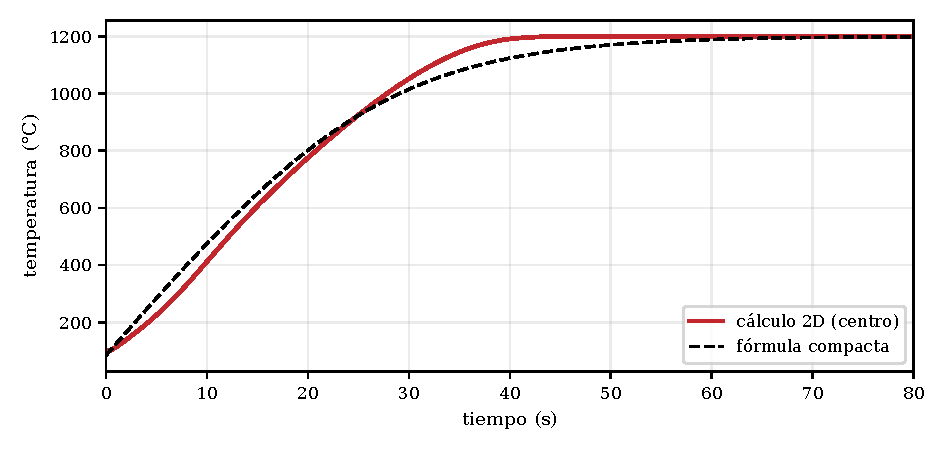
\includegraphics[width=\linewidth]{fig_compacta.pdf}
\caption{Temperatura del centro según el cálculo bidimensional y según la
fórmula compacta, para la pastilla de referencia en contacto puntual y horno
ideal. La fórmula ignora el canto, que en esta geometría supone el
\SI{37}{\percent} del área expuesta, y por eso va por detrás.}
\end{figure}

Con soporte, la fórmula no es aplicable. El soporte añade una masa térmica
que hay que calentar y bloquea una de las dos caras radiantes; ninguno de
los dos efectos cabe en un modelo de un solo grado de libertad. En ese caso
sirve únicamente como cota inferior: el tiempo que se alcanzaría si se
eliminase el soporte.

% ==========================================================================
\section{Magnitudes derivadas}

\subsection{Velocidad de calentamiento}

La literatura de sinterización rápida se expresa en \si{\kelvin\per\minute}
o \si{\kelvin\per\second}, de modo que la velocidad del punto más frío es la
magnitud que permite situar un ensayo frente a la bibliografía:

\begin{equation}
\dot{T}_{c}(t) = \frac{\mathrm{d}T_{c}}{\mathrm{d}t}
\end{equation}

Conviene una advertencia numérica. Si esta derivada se evalúa sobre la curva
almacenada para representación, el valor de pico depende del intervalo de
muestreo y lo subestima apreciablemente. En el caso de referencia, el máximo
pasaba de \num{55} a \SI{67.5}{\kelvin\per\second} al aumentar el número de
puntos guardados. La derivada debe calcularse sobre el paso de tiempo propio
del integrador.

\subsection{Tensión de origen térmico}

Una pieza con gradiente térmico se dilata como un conjunto. Cada punto
queda traccionado o comprimido según se aparte de la deformación media, de
manera que el motor de la tensión no es la diferencia entre la cara y el
centro, sino entre cada punto y la temperatura \emph{media} de la pieza.
Para una placa con gradiente en el espesor y bordes libres:

\begin{equation}
\boxed{\;
\sigma(x) = \frac{E \cdot \alpha_{t}}{1 - \nu}
\left( T_{m} - T(x) \right)
\;}
\end{equation}

El factor $1/(1-\nu)$ aparece porque la dilatación está impedida en las dos
direcciones del plano de la placa, no en una sola. Durante el calentamiento
el centro queda por debajo de la media y entra en \emph{tracción}, que es el
modo en que fallan las cerámicas, mientras la superficie queda comprimida.

El valor debe leerse como orden de magnitud. En verde, el módulo de Young es
muy inferior al de la pieza densa, de modo que la tensión real es menor que
la calculada con propiedades de material denso, pero también lo es la
resistencia. La utilidad del cálculo está en comparar montajes, no en
predecir la rotura.

% ==========================================================================
\section{Propiedades de los materiales}
\label{sec:propiedades}

Todas las propiedades térmicas y ópticas se introducen como función de la
temperatura absoluta, en kelvin. El modelo las trata según se describe en el
apartado \ref{sec:entalpia}.

\subsection{Electrolito: LATP}

\begin{equation}
\begin{aligned}
k(T) &= -2{,}016\cdot10^{-17}\,T^{6} + 1{,}278\cdot10^{-13}\,T^{5}
      - 3{,}236\cdot10^{-10}\,T^{4} \\
     &\quad + 4{,}090\cdot10^{-7}\,T^{3} - 2{,}673\cdot10^{-4}\,T^{2}
      + 8{,}585\cdot10^{-2}\,T - 9{,}700
\end{aligned}
\end{equation}

\begin{equation}
\begin{aligned}
c_p(T) &= -6{,}414\cdot10^{-14}\,T^{6} + 3{,}680\cdot10^{-10}\,T^{5}
        - 8{,}507\cdot10^{-7}\,T^{4} \\
       &\quad + 9{,}983\cdot10^{-4}\,T^{3} - 6{,}179\cdot10^{-1}\,T^{2}
        + 1{,}899\cdot10^{2}\,T - 2{,}091\cdot10^{4}
\end{aligned}
\end{equation}

\begin{equation}
\varepsilon(T) = 5{,}600\cdot10^{-4}\,T + 1{,}210\cdot10^{-1}
\qquad
\alpha(T) = 9{,}774\cdot10^{-11}\,T + 1{,}486\cdot10^{-7}
\end{equation}

La emisividad y el calor específico proceden de medidas propias: la primera
con pirómetro en el laboratorio, el segundo según se recoge en el artículo
sobre sinterización rápida. La conductividad no es una medida independiente:
se obtiene a partir de la linealización de los valores medidos de
difusividad y su posterior ajuste a un polinomio de sexto grado.

\subsection{Soporte: alúmina}

\begin{equation}
k(T) = 1{,}912\cdot10^{-5}\,T^{2} - 5{,}025\cdot10^{-2}\,T + 3{,}866\cdot10^{1}
\end{equation}

\begin{equation}
c_p(T) = 9{,}052\cdot10^{2} + 3{,}678\cdot10^{-1}\,T
         - 2{,}142\cdot10^{-3}\,T^{-2}
\end{equation}

\begin{equation}
\varepsilon(T) = 7{,}314\cdot10^{-4}\,T - 1{,}774\cdot10^{-1}
\end{equation}

El calor específico procede de \emph{Tablas cerámicas} (Enrique Navarro,
1984) y la conductividad del \emph{CRC Handbook of Materials Science and
Engineering}. La emisividad se ha medido en el laboratorio con pirómetro,
igual que la del LATP.

\begin{figure}[htbp]
\centering
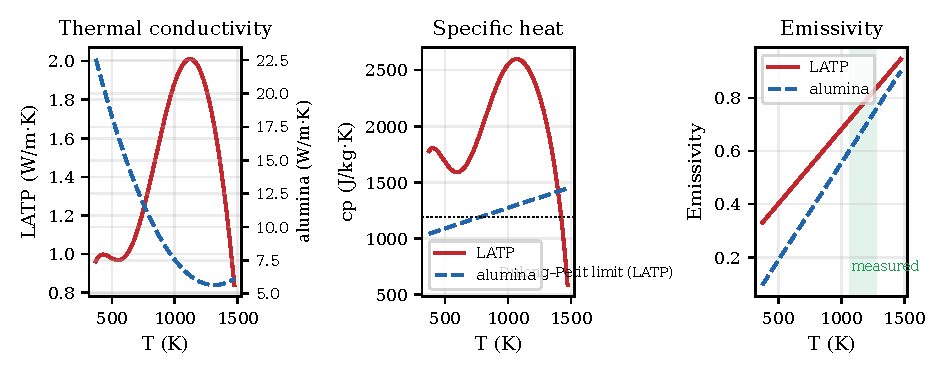
\includegraphics[width=\linewidth]{fig_props.pdf}
\caption{Las seis funciones empleadas, en su rango de validez. La línea de
puntos del panel central marca el límite de Dulong y Petit para el LATP,
que el ajuste del calor específico supera en todo el intervalo; la banda
verde del panel derecho señala el intervalo en que se midió la emisividad,
fuera del cual las rectas son extrapolación.}
\end{figure}

\subsection{Coherencia interna y densidad del LATP}

Las tres funciones medidas del LATP no son independientes entre sí, puesto
que la conductividad se dedujo de la difusividad. Esa dependencia permite
una comprobación: si todas son mutuamente consistentes, el cociente

\begin{equation}
\rho = \frac{k(T)}{\alpha(T) \cdot c_p(T)}
\end{equation}

debe resultar constante. Evaluado entre \SI{400}{\kelvin} y
\SI{1200}{\kelvin} da \SI{2990}{\kilogram\per\meter\cubed} con una
dispersión del \SI{3}{\percent}, valor coherente con un LATP denso. La
densidad empleada en el modelo es esa, y no un dato independiente.

\subsection{Rango de validez y recorte}

Fuera del intervalo \SIrange{373}{1473}{\kelvin} los ajustes dejan de tener
sentido físico, como recoge la \tab{2}. Los polinomios de sexto grado del
LATP cruzan el cero y se vuelven negativos por encima de
\SI{1500}{\kelvin}, y ambas emisividades superan la unidad por encima de
\SI{1570}{\kelvin}. El modelo mantiene por ello el valor del extremo fuera
del rango declarado, en lugar de extrapolar.

\begin{table}[htbp]
\centering
\caption*{\textcolor{uji}{\textbf{Tabla 2.}} Comportamiento de los ajustes
dentro y fuera del rango de validez.}
\begin{tabular}{lccc}
\toprule
Función & \SI{373}{\kelvin} & \SI{1473}{\kelvin} & Fuera de rango \\
\midrule
$k$ LATP & \num{0.96} & \num{0.84} & $<0$ por encima de \SI{1540}{\kelvin} \\
$c_p$ LATP & \num{1779} & \num{585} & $<0$ por encima de \SI{1510}{\kelvin} \\
$\varepsilon$ LATP & \num{0.33} & \num{0.95} & $>1$ por encima de \SI{1570}{\kelvin} \\
$k$ alúmina & \num{22.6} & \num{6.1} & mínimo en \SI{1314}{\kelvin} \\
$c_p$ alúmina & \num{1042} & \num{1447} & monótona \\
$\varepsilon$ alúmina & \num{0.10} & \num{0.90} & $>1$ por encima de \SI{1610}{\kelvin} \\
\bottomrule
\end{tabular}
\end{table}

\subsection{Dos reservas sobre los datos}
\label{sec:reservas}

\textbf{El calor específico del LATP excede el límite clásico.} El valor
máximo que puede alcanzar el calor específico de un sólido cristalino por
agitación térmica lo fija la ley de Dulong y Petit, que asigna $3R$ por mol
de átomos:

\begin{equation}
c_{p,\max} = \frac{3R \cdot n_{\text{átomos}}}{M}
= \frac{3 \cdot 8{,}314 \cdot 18{,}3}{0{,}3834}
\approx \SI{1190}{\joule\per\kilogram\per\kelvin}
\end{equation}

para Li$_{1,3}$Al$_{0,3}$Ti$_{1,7}$(PO$_4$)$_3$, de masa molar
\SI{383.4}{\gram\per\mole} y \num{18.3} átomos por fórmula. El ajuste
empleado da entre \num{1.4} y \num{2.2} veces ese límite en todo el
intervalo de trabajo, con un máximo de
\SI{2598}{\joule\per\kilogram\per\kelvin} a \SI{1073}{\kelvin}.

Un calor específico \emph{sensible} no puede superar ese techo. La lectura
compatible con el dato es que se trate de un calor específico
\emph{aparente}, obtenido por calorimetría diferencial durante el
calentamiento, que incorpora la entalpía de las transformaciones que ocurren
en ese intervalo. Si es así, el dato es legítimo y el modelo lo trata
correctamente: la formulación entálpica del apartado \ref{sec:entalpia}
absorbe sin modificación cualquier calor latente. Conviene, en todo caso,
nombrarlo como calor específico aparente y no compararlo con valores
tabulados de calor sensible.

\textbf{El término en $T^{-2}$ del calor específico de la alúmina es
numéricamente nulo.} Con el coeficiente $2{,}142\cdot10^{-3}$ ese sumando
vale $-1{,}5\cdot10^{-8}$ a \SI{373}{\kelvin}, esto es, diez órdenes de
magnitud por debajo del resto de la expresión. Los ajustes del tipo
Maier--Kelley para la alúmina llevan en esa posición un coeficiente del
orden de $10^{7}$; con él, el calor específico a \SI{373}{\kelvin} pasaría
de \num{1042} a \SI{888}{\joule\per\kilogram\per\kelvin}, que es el valor
habitualmente tabulado. Procede verificar el exponente en la fuente
original.

% ==========================================================================
\section{Resultados del caso de referencia}

\subsection{Evolución térmica}

La \fig{4} recoge la evolución de la temperatura en los puntos
característicos de la pieza. El soporte, que parte frío y tiene una masa
térmica considerable, se calienta más despacio que la muestra y actúa como
sumidero sobre su cara inferior durante todo el transitorio.

\begin{figure}[htbp]
\centering
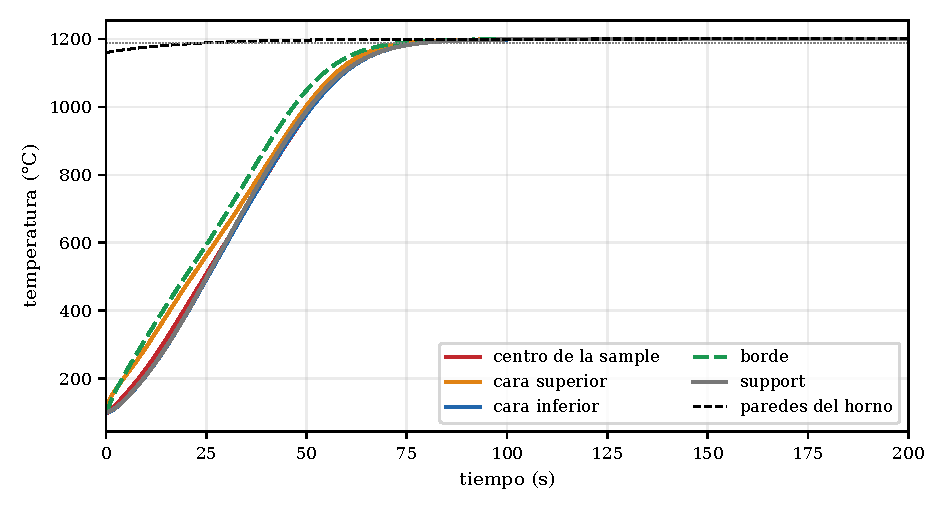
\includegraphics[width=\linewidth]{fig_curvas.pdf}
\caption{Evolución de la temperatura en el centro, las caras, el borde y el
soporte, frente a la temperatura de las paredes del horno. La línea de
puntos marca el \SI{99}{\percent} del salto térmico.}
\end{figure}

\begin{table}[htbp]
\centering
\caption*{\textcolor{uji}{\textbf{Tabla 3.}} Resultados del caso de
referencia: pastilla de LATP de \SI{10}{\milli\meter} de diámetro y
\SI{1.5}{\milli\meter} de espesor sobre soporte de alúmina de
\SI{3}{\milli\meter}, introducida a \SI{100}{\celsius} en un horno a
\SI{1200}{\celsius}.}
\begin{tabular}{lll}
\toprule
Magnitud & Valor & Observación \\
\midrule
$t_{50}$ del centro & \SI{32.4}{\second} & \\
$t_{90}$ del centro & \SI{58.2}{\second} & \\
$t_{99}$ del centro & \SI{78.3}{\second} & tiempo de puesta a régimen \\
Desfase cara--centro & \SI{68}{\kelvin} & máximo del transitorio \\
Desfase media--centro & \SI{52}{\kelvin} & motor de la tensión \\
Velocidad máxima & \SI{19.5}{\kelvin\per\second} & \SI{1170}{\kelvin\per\minute} \\
Tracción máxima en el centro & \SI{70}{\mega\pascal} & con propiedades de material denso \\
$h_{rad}$ medio & \SI{262}{\watt\per\meter\squared\per\kelvin} & frente a \SI{10}{} de convección \\
$Bi$ & \num{0.141} & por encima del límite de \num{0.1} \\
$\tau$ & \SI{16.4}{\second} & constante de tiempo \\
Paso de tiempo & \SI{0.39}{\milli\second} & malla $16 \times 33$ \\
\bottomrule
\end{tabular}
\end{table}

La \fig{5} muestra los perfiles internos. El perfil axial es
\emph{monótono y fuertemente asimétrico}: la cara superior, que ve el horno,
va siempre por delante, y la inferior queda retrasada por el contacto con el
soporte frío. Conviene subrayar que esto no contradice la hipótesis de
perfil parabólico de la sección \ref{sec:agrupado}, pero sí acota su
alcance: aquella parábola es simétrica y supone calentamiento por las dos
caras, de modo que describe el caso de contacto puntual, no el de una pieza
apoyada sobre un soporte macizo. Es una razón más por la que la fórmula
compacta no es aplicable con soporte.

El perfil radial, en cambio, es casi plano salvo en una franja próxima al
borde, tal como anticipaba la estimación de escalas de la \ecu{6}.

\begin{figure}[htbp]
\centering
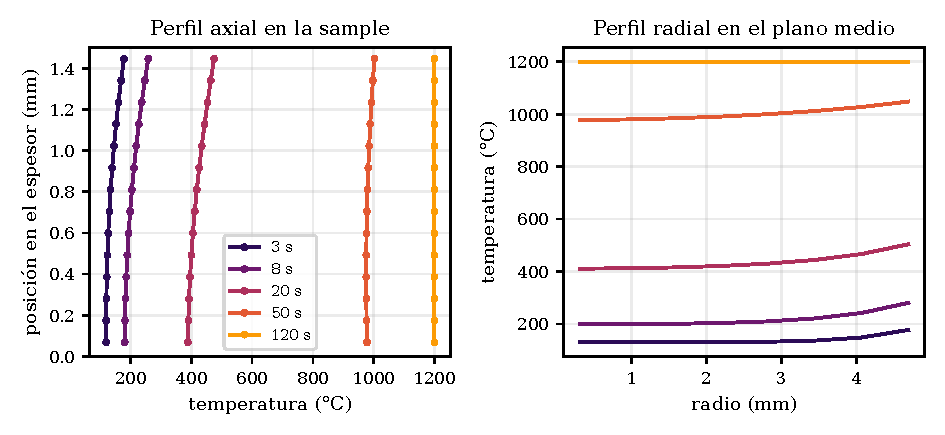
\includegraphics[width=\linewidth]{fig_perfiles.pdf}
\caption{Perfiles de temperatura en el espesor de la muestra, sobre el eje,
y en el radio, sobre el plano medio, en distintos instantes. La cota
\SI{0}{\milli\meter} es la cara en contacto con el soporte y
\SI{1.5}{\milli\meter} la que ve el horno. Los puntos señalan los nodos de
la malla.}
\end{figure}

\subsection{Velocidad y tensión}

\begin{figure}[htbp]
\centering
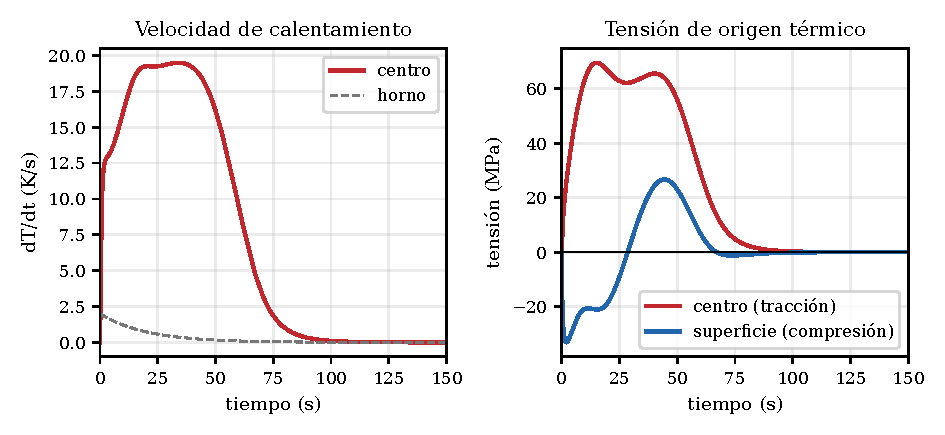
\includegraphics[width=\linewidth]{fig_velocidad.pdf}
\caption{Velocidad de calentamiento del centro y tensión de origen térmico.
El centro trabaja a tracción y la superficie a compresión, con el máximo en
los primeros segundos.}
\end{figure}

La velocidad máxima del centro, \SI{1170}{\kelvin\per\minute}, sitúa el
ensayo en el régimen de sinterización rápida, aunque lejos de los valores
que se obtendrían con una masa térmica menor. El máximo de tensión no
coincide con el de velocidad sino que se alcanza unos segundos después,
cuando el gradiente interno es mayor.

\subsection{Comparación con una rampa programada}

La \fig{7} enfrenta la introducción directa en el horno caliente con una
rampa convencional de \SI{600}{\celsius\per\minute} hasta la misma
consigna.

\begin{figure}[htbp]
\centering
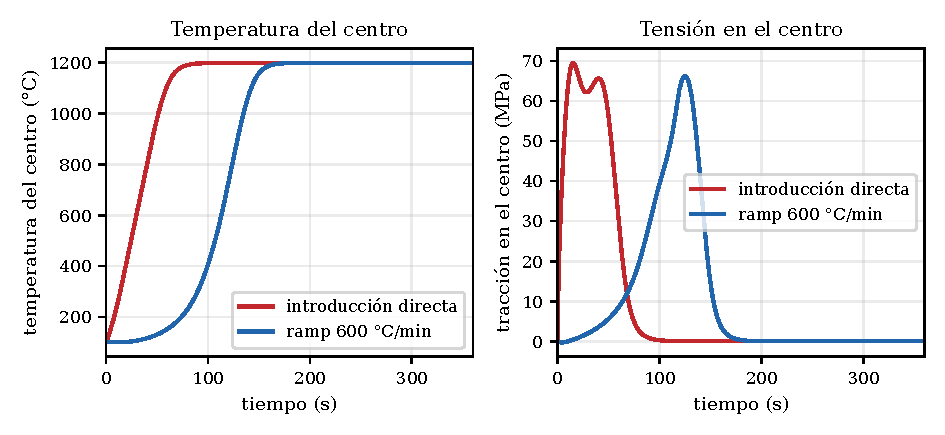
\includegraphics[width=\linewidth]{fig_rampa.pdf}
\caption{Introducción directa frente a rampa programada de
\SI{600}{\celsius\per\minute}: temperatura del centro y tensión asociada.}
\end{figure}

\begin{table}[htbp]
\centering
\caption*{\textcolor{uji}{\textbf{Tabla 4.}} Comparación de los dos
programas térmicos.}
\begin{tabular}{lcc}
\toprule
 & Introducción directa & Rampa de \SI{600}{\celsius\per\minute} \\
\midrule
$t_{99}$ del centro & \SI{78.3}{\second} & \SI{160.6}{\second} \\
Velocidad máxima & \SI{19.5}{\kelvin\per\second} & \SI{19.5}{\kelvin\per\second} \\
Desfase cara--centro & \SI{68}{\kelvin} & \SI{39}{\kelvin} \\
Tracción en el centro & \SI{70}{\mega\pascal} & \SI{66}{\mega\pascal} \\
\bottomrule
\end{tabular}
\end{table}

Con las propiedades medidas el canje habitual de la sinterización rápida
casi desaparece: la introducción directa es el doble de rápida y la tensión
apenas sube, de \SI{66}{\mega\pascal} a \SI{70}{\mega\pascal}. La razón está
en el número de Biot, que con estas propiedades vale \num{0.141}: la
pastilla está cerca de ser isoterma, de modo que acelerar el calentamiento
no genera gradientes internos apreciables. El factor limitante no es la
conducción dentro de la pieza, sino la energía que hay que suministrarle.

% ==========================================================================
\section{Validación del código}

\subsection{Contraste con la solución analítica}

El caso de prueba es la placa plana infinita con convección superficial,
cuya solución exacta en serie es conocida\cita{2,1}:

\begin{equation}
\theta = \frac{T - T_{\infty}}{T_{0} - T_{\infty}}
= \sum_{n=1}^{\infty} C_{n}\, e^{-\lambda_{n}^{2} Fo}
  \cos\left( \lambda_{n}\, \frac{x}{L} \right)
\end{equation}

donde los autovalores $\lambda_{n}$ son las raíces de la ecuación
trascendente que impone la condición de contorno convectiva, y los
coeficientes proceden de la ortogonalidad de los modos:

\begin{equation}
\lambda_{n} \tan \lambda_{n} = Bi
\qquad
C_{n} = \frac{4 \sin \lambda_{n}}
             {2 \lambda_{n} + \sin\left( 2 \lambda_{n} \right)}
\qquad
Fo = \frac{\alpha \cdot t}{L^{2}}
\end{equation}

El número de Fourier $Fo$ es el tiempo adimensional del problema: compara el
tiempo transcurrido con el tiempo característico de difusión $L^{2}/\alpha$.

La prueba se realiza con $Bi = 1$, desactivando la radiación y empleando un
cilindro suficientemente ancho para que el eje se comporte como una placa.
Sumando veinte términos de la serie, el error máximo para $Fo > \num{0.05}$
se recoge en la \tab{5}. El contraste verifica simultáneamente la
discretización espacial, el tratamiento de la superficie y el paso de
tiempo.

\begin{table}[htbp]
\centering
\caption*{\textcolor{uji}{\textbf{Tabla 5.}} Error máximo frente a la serie
analítica, en porcentaje del salto térmico total, al refinar la malla.}
\begin{tabular}{ccc}
\toprule
Celdas en el semiespesor & Error máximo & Razón respecto al anterior \\
\midrule
\num{10} & \SI{0.338}{\percent} & --- \\
\num{20} & \SI{0.084}{\percent} & \num{4.0} \\
\num{40} & \SI{0.021}{\percent} & \num{4.0} \\
\num{80} & \SI{0.0053}{\percent} & \num{4.0} \\
\bottomrule
\end{tabular}
\end{table}

El error se divide exactamente por cuatro cada vez que se duplica el número
de celdas. Ese factor es la firma de un esquema de \emph{segundo orden} en
el espacio, que es lo que corresponde a una discretización por volúmenes
finitos centrada: el error debe escalar como $\Delta z^{2}$. La convergencia
observada confirma que la implementación no contiene errores de primer orden
ocultos, lo que un único cálculo contrastado nunca podría demostrar.

Merece la pena señalar que la aproximación de un solo término de la serie,
válida solo para $Fo > \num{0.2}$, difiere del cálculo completo en un
\SI{1.4}{\percent}: un contraste riguroso exige la serie entera.

\subsection{Independencia de malla}

Verificar la convergencia frente a una solución exacta no basta, porque el
caso real incluye dos materiales y una condición radiativa. Se repiten por
ello cuatro configuraciones con tres resoluciones, entre \num{8} y \num{22}
celdas en el espesor de la muestra.

\begin{table}[htbp]
\centering
\caption*{\textcolor{uji}{\textbf{Tabla 6.}} Tiempo hasta el
\SI{99}{\percent} del salto térmico en el centro, para tres resoluciones de
malla. Pastilla de \SI{10}{\milli\meter} de diámetro.}
\begin{tabular}{lcccc}
\toprule
Montaje & 8 celdas & 14 celdas & 22 celdas & Dispersión \\
\midrule
Contacto puntual                 & \SI{43.8}{\second} & \SI{43.7}{\second} & \SI{43.7}{\second} & \SI{0.2}{\percent} \\
Soporte de \SI{1}{\milli\meter}  & \SI{58.1}{\second} & \SI{55.7}{\second} & \SI{56.1}{\second} & \SI{4.3}{\percent} \\
Soporte de \SI{2}{\milli\meter}  & \SI{80.8}{\second} & \SI{78.3}{\second} & \SI{77.6}{\second} & \SI{4.1}{\percent} \\
Soporte de \SI{5}{\milli\meter}  & \SI{138.9}{\second} & \SI{136.8}{\second} & \SI{135.9}{\second} & \SI{2.2}{\percent} \\
\bottomrule
\end{tabular}
\end{table}

La dispersión llega ahora al \SI{4}{\percent}, frente al \SI{1}{\percent}
que se obtenía con propiedades constantes. El motivo es el redondeo del
número de celdas con que se representa el soporte, que con propiedades
dependientes de la temperatura desplaza además el punto en que se evalúan.
La malla intermedia es la que se emplea en los resultados; la más gruesa
sigue siendo suficiente para explorar tendencias, que es lo que abarata el
análisis de sensibilidad de la sección siguiente.

\subsection{Alcance de la validación}

La validación confirma que las ecuaciones planteadas se resuelven
correctamente. No confirma que sean las ecuaciones correctas para un horno
concreto. Esto último exige una medida experimental, y se discute a
continuación.

% ==========================================================================
\section{Análisis de sensibilidad}

\subsection{Elasticidad como indicador}

Un modelo con diecisiete variables de entrada no es útil si no se sabe
cuáles gobiernan el resultado. El indicador adecuado para compararlas no es
la derivada $\partial t_{99}/\partial x$, porque sus unidades dependen de la
variable y su valor numérico, de la elección de unidades. Se emplea en su
lugar la \emph{elasticidad}, que es la derivada en escala logarítmica y por
tanto adimensional:

\begin{equation}
\boxed{\;
S = \frac{\mathrm{d}\left( \ln t_{99} \right)}
         {\mathrm{d}\left( \ln x \right)}
= \frac{\Delta t_{99} / t_{99}}{\Delta x / x}
\;}
\end{equation}

Su lectura es directa: $S = 1$ indica proporcionalidad, de modo que duplicar
la variable duplica el tiempo; $S = 0$ indica que la variable no influye; un
valor negativo indica que al aumentar la variable disminuye el tiempo.
Equivalentemente, duplicar una variable multiplica el tiempo por $2^{S}$.

En la práctica se evalúa por diferencias centradas:

\begin{equation}
S \approx \frac{\ln t_{99}(x^{+}) - \ln t_{99}(x^{-})}
               {\ln x^{+} - \ln x^{-}}
\end{equation}

\subsection{Una precaución metodológica}

La perturbación empleada es del \SI{\pm 22}{\percent}, deliberadamente
amplia. Con perturbaciones pequeñas, del orden del \SI{\pm 5}{\percent}, el
resultado de las variables débiles queda enterrado en el ruido de
discretización: al modificar un espesor cambia el número de celdas con que
se representa el soporte, y puesto que la masa del soporte tiene una
elasticidad próxima a \num{0.6}, ese redondeo introduce saltos del orden del
\SI{1}{\percent} en $t_{99}$, del mismo orden que la señal buscada. Con
\SI{\pm 5}{\percent} el espesor de la muestra llegaba a salir con signo
negativo, en contradicción con el barrido amplio. Las elasticidades que
siguen son, por tanto, secantes sobre un intervalo finito y no derivadas
puntuales.

\subsection{Resultados}

\begin{figure}[htbp]
\centering
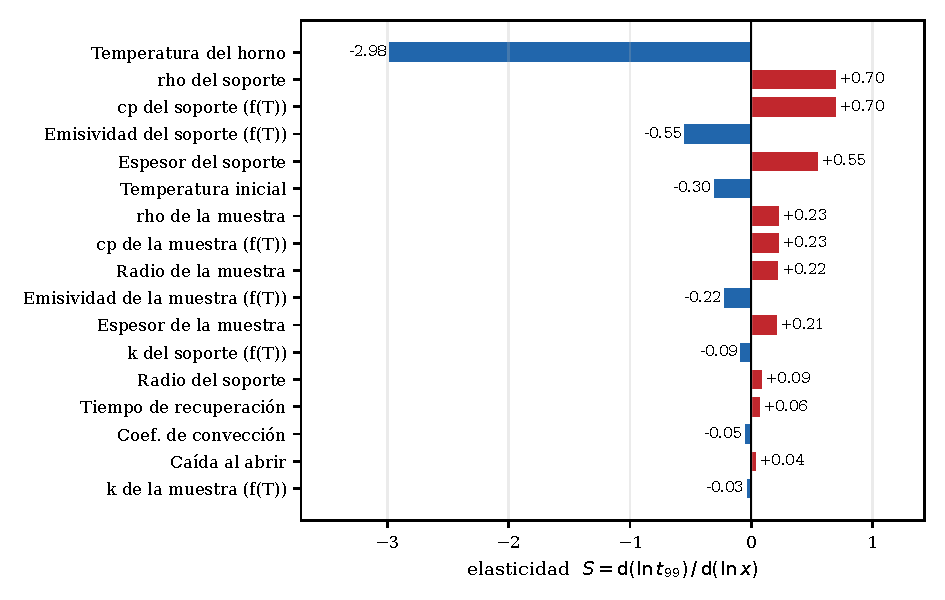
\includegraphics[width=\linewidth]{fig_tornado.pdf}
\caption{Elasticidad del tiempo de calentamiento respecto de cada variable
de entrada. En rojo, las que lo alargan al aumentar; en azul, las que lo
acortan.}
\end{figure}

Con las propiedades medidas, el reparto de influencias cambia respecto al
que se obtiene con propiedades constantes. El soporte y el horno siguen
dominando, pero la muestra ha dejado de ser irrelevante.

La densidad y el calor específico del soporte dan exactamente la misma
elasticidad, $S = \num{0.696}$, porque solo intervienen a través de su
producto $\rho_{s} \cdot c_{p,s}$, que es su capacidad térmica por unidad de
volumen. Lo mismo ocurre en la muestra, con $S = \num{0.225}$ en ambas. Es
el modelo confirmando su propia estructura, y constituye una comprobación
interna útil: el calor específico entra como función de $T$ y la densidad
como constante, y aun así ambas salen con idéntica elasticidad.

\subsection{Lo que cambia respecto a las propiedades de literatura}

Con los valores constantes de literatura, ninguna propiedad de la muestra
alcanzaba una elasticidad de \num{0.14}. Con las propiedades medidas, cuatro
magnitudes de la muestra superan \num{0.2}: su capacidad térmica, su radio,
su emisividad y su espesor. El motivo es que la capacidad térmica
volumétrica del LATP medido, $\rho \cdot c_p \approx
\SI{7.2e6}{\joule\per\meter\cubed\per\kelvin}$, cuadruplica la que se
suponía. La muestra ha pasado de ser un pasajero a aportar una fracción
apreciable de la energía que hay que suministrar.

La consecuencia práctica es que la discusión del apartado
\ref{sec:reservas} sobre el calor específico deja de ser académica. Con
$S = \num{0.225}$, un factor dos en $c_p$ mueve el tiempo de calentamiento
un \SI{17}{\percent}, y el gradiente interno bastante más.

\subsection{Lo que sigue sin importar}

Tres resultados negativos se mantienen, y evitan trabajo inútil:

\begin{itemize}
\item La \emph{resistencia térmica de contacto} es irrelevante en todo el
rango realista: haría falta una resistencia un orden de magnitud mayor para
competir con la radiación.

\item La \emph{convección} no cuenta, con $S = \num{-0.049}$. A
\SI{1200}{\celsius} el coeficiente radiativo es unas veintiséis veces el
convectivo.

\item La \emph{conductividad} de ambos materiales apenas influye:
$S = \num{-0.033}$ para el LATP y $S = \num{-0.086}$ para la alúmina. Con un
número de Biot de \num{0.141}, la pieza está cerca de ser isoterma y la
resistencia interna aporta poco al total.
\end{itemize}

Esto ordena las prioridades experimentales. Lo que conviene medir con
cuidado es la emisividad del soporte, su masa térmica y la curva real de
recuperación del horno; y, a la luz del cambio anterior, confirmar la
naturaleza del calor específico del LATP.

% ==========================================================================
\section{Hipótesis, limitaciones y vías de mejora}
\label{sec:limitaciones}

\subsection{Inventario de hipótesis}

La \tab{7} reúne las hipótesis adoptadas junto con el orden de magnitud de lo que cada una descarta. Una hipótesis sin su cota es una declaración de intenciones, no un argumento.

\begin{table}[htbp]
\centering
\caption*{\textcolor{uji}{\textbf{Tabla 7.}} Hipótesis del modelo y orden de
magnitud de lo que cada una descarta.}
\begin{tabular}{p{4.4cm}p{5.6cm}p{3.6cm}}
\toprule
Hipótesis & Fundamento & Efecto estimado \\
\midrule
Simetría axial & Geometría y contorno independientes del ángulo & Exacta con calentamiento uniforme \\
Propiedades constantes con $T$ & \emph{Ya no se aplica}: $k$, $c_p$ y $\varepsilon$ entran como función de $T$ & Queda la dependencia con la porosidad \\
Cuerpo gris, factor de forma unidad & Cuerpo pequeño en cavidad grande & No contempla el apantallamiento del borde \\
Superficie opaca & Dispersión intensa en un cuerpo poroso & Pequeño, no verificado \\
Sin calor de sinterización & Latente frente a sensible & $\sim\SI{1}{\percent}$ \\
Geometría fija & La contracción ocurre tras la rampa & $\sim\SI{1}{\percent}$ \\
Ley de Fourier & Relajación fonónica $\sim$ ps & Exacta a esta escala \\
$h_c$ constante & No acoplado al campo de temperaturas & La convección aporta $\sim\SI{3}{\percent}$ \\
\bottomrule
\end{tabular}
\end{table}

\subsection{La limitación principal: la geometría radiativa}

La hipótesis de factor de forma unidad es la debilidad seria del modelo. El
soporte sobresale varios milímetros más allá del borde de la pastilla, de
modo que \emph{apantalla el canto} en los ángulos rasantes: ese canto ve
parcialmente la cara superior del soporte, más fría, en lugar de las paredes
del horno. Y el canto no es un detalle geométrico: con
\SI{10}{\milli\meter} de diámetro y \SI{1.5}{\milli\meter} de espesor,
supone el \SI{37}{\percent} del área expuesta de la pastilla.

\begin{equation}
\frac{A_{canto}}{A_{total}}
= \frac{2\pi\, R\, e}{\pi\, R^{2} + 2\pi\, R\, e}
= \frac{e}{R/2 + e}
\end{equation}

El modelo actual calienta ese canto de más. La solución rigurosa pasa por un
método de radiosidad con factores de forma entre las cuatro superficies que
intervienen: cara superior de la muestra, canto, cara superior del soporte y
paredes del horno. Es el único cambio de modelado capaz de mover el
resultado más de un \SI{10}{\percent}.

\subsection{Otras limitaciones}

\begin{itemize}
\item \emph{Condición en la base del soporte}. El modelo supone que la cara
inferior del soporte radia hacia el horno. Si en la práctica descansa sobre
la solera, está conduciendo hacia una masa mucho mayor y el sumidero
térmico es considerablemente más grande.

\item \emph{Opacidad}. A \SI{1200}{\celsius} el máximo de emisión cae en
\SI{2}{\micro\meter}, donde muchos óxidos son parcialmente transparentes. La
intensa dispersión de un cuerpo poroso limita la penetración, pero el efecto
no está cuantificado.

\item \emph{Programa del horno}. Los valores de $\Delta T$ y $\tau_{h}$ son
estimaciones. Influyen poco en el tiempo total, pero gobiernan por completo
la parte inicial de la curva, que es la que fija la velocidad de
calentamiento.
\end{itemize}

\subsection{La acción de mayor valor}

Un termopar fino embebido en una pastilla de sacrificio, registrando la
introducción en el horno, calibra simultáneamente la emisividad efectiva, la
geometría radiativa y la recuperación del horno. Cualquier refinamiento de
modelado emprendido sin esa medida equivale a pulir la parte del trabajo que
ya funciona.

% ==========================================================================
\section{Nomenclatura}

\begin{table}[htbp]
\centering
\caption*{\textcolor{uji}{\textbf{Tabla 8.}} Símbolos, unidades y valores de
referencia.}
\begin{tabular}{llll}
\toprule
Símbolo & Magnitud & Unidad & Valor de referencia \\
\midrule
$T$ & Temperatura & \si{\kelvin} & --- \\
$T_c, T_s, T_m$ & Centro, pared y media & \si{\kelvin} & --- \\
$T_h$ & Paredes del horno & \si{\kelvin} & \num{1473} \\
$T_0$ & Inicial de la muestra & \si{\kelvin} & \num{373} \\
$e$ & Espesor de la muestra & \si{\meter} & \num{1.5e-3} \\
$L$ & Semiespesor, $e/2$ & \si{\meter} & \num{0.75e-3} \\
$R$ & Radio de la muestra & \si{\meter} & \num{5e-3} \\
$e_s$ & Espesor del soporte & \si{\meter} & \num{2e-3} \\
$k$ & Conductividad térmica & \si{\watt\per\meter\per\kelvin} & $f(T)$, sección \ref{sec:propiedades} \\
$\rho$ & Densidad & \si{\kilogram\per\meter\cubed} & \num{2990} / \num{3900} \\
$c_p$ & Calor específico & \si{\joule\per\kilogram\per\kelvin} & $f(T)$, sección \ref{sec:propiedades} \\
$\alpha$ & Difusividad, $k/(\rho c_p)$ & \si{\meter\squared\per\second} & \numrange{1.9e-7}{2.9e-7} \\
$\varepsilon$ & Emisividad & --- & $f(T)$, sección \ref{sec:propiedades} \\
$\sigma$ & Constante de Stefan--Boltzmann & \si{\watt\per\meter\squared\per\kelvin\tothe{4}} & \num{5.670e-8} \\
$h_c$ & Coeficiente de convección & \si{\watt\per\meter\squared\per\kelvin} & \num{10} \\
$h_{rad}$ & Coeficiente radiativo equivalente & \si{\watt\per\meter\squared\per\kelvin} & \num{262} \\
$R_c$ & Resistencia de contacto & \si{\meter\squared\kelvin\per\watt} & \num{0} \\
$E$ & Módulo de Young & \si{\pascal} & \num{100e9} \\
$\alpha_t$ & Coeficiente de dilatación & \si{\per\kelvin} & \num{1e-5} \\
$\nu$ & Coeficiente de Poisson & --- & \num{0.25} \\
$Bi$ & Número de Biot, $hL/k$ & --- & \num{0.141} \\
$Fo$ & Número de Fourier, $\alpha t/L^2$ & --- & --- \\
$\tau$ & Constante de tiempo, $\rho c_p L/h$ & \si{\second} & \num{16.4} \\
$q''$ & Flujo de calor por unidad de área & \si{\watt\per\meter\squared} & --- \\
$G$ & Conductancia entre celdas & \si{\watt\per\kelvin} & --- \\
\bottomrule
\end{tabular}
\end{table}

Las propiedades del LATP y la emisividad de la alúmina proceden de medidas
propias; el resto, de literatura. Sus expresiones y sus fuentes se recogen
en la sección \ref{sec:propiedades}.

% ==========================================================================
\begin{thebibliography}{9}
\small
\bibitem{incropera} F. P. Incropera, D. P. DeWitt, T. L. Bergman,
A. S. Lavine. \emph{Fundamentals of Heat and Mass Transfer}, 7.\textsuperscript{a}
ed. Wiley, 2011.
\bibitem{carslaw} H. S. Carslaw, J. C. Jaeger. \emph{Conduction of Heat in
Solids}, 2.\textsuperscript{a} ed. Oxford University Press, 1959.
\bibitem{patankar} S. V. Patankar. \emph{Numerical Heat Transfer and Fluid
Flow}. Hemisphere Publishing, 1980.
\bibitem{ozisik} M. N. Özişik. \emph{Heat Conduction}, 2.\textsuperscript{a}
ed. Wiley, 1993.
\bibitem{modest} M. F. Modest. \emph{Radiative Heat Transfer},
3.\textsuperscript{a} ed. Academic Press, 2013.
\bibitem{mills} A. F. Mills. \emph{Heat and Mass Transfer}. Irwin, 1995.
\bibitem{versteeg} H. K. Versteeg, W. Malalasekera. \emph{An Introduction to
Computational Fluid Dynamics: The Finite Volume Method},
2.\textsuperscript{a} ed. Pearson, 2007.
\bibitem{siegel} R. Siegel, J. R. Howell. \emph{Thermal Radiation Heat
Transfer}, 4.\textsuperscript{a} ed. Taylor \& Francis, 2002.
\end{thebibliography}

\end{document}
